\documentclass[12pt, oneside]{article}
\usepackage{amsfonts}
\usepackage{cite}
\usepackage{graphicx}
\graphicspath{ {images/} }
\begin{document}
\begin{titlepage}
\begin{center}
\vspace*{1cm}
{\Huge Universitatea Alexandru Ioan Cuza Iași} \\
\vspace{0.5cm}
{\huge \textbf{Facultatea de Informatică}} \\
\vspace{1.5cm}

\includegraphics[width=3cm,height=4.5cm,keepaspectratio]{logo_fii3.png} \\
\vspace{1cm}
TAIP Project \\ 
\vspace{0.5cm}
{\Huge \textbf{Service Orchestration}} \\
\vspace{1cm}


\vspace{1cm}
\end{center}
\end{titlepage}
	\section{What is service orchestration}
	Service orchestration is the coordination and arrangement of multiple services exposed as a single aggregate service. Developers utilize service orchestration to support the automation of business procceses by loosely coupling services across different applications and enterprises and creating composite applications. In other words, service orchestration is the combination of service interactions to create higher-level business services. This works through the exchange of messages in the domain layer of enterprise applications. Since individual services are not programmed to cummunicate with other services, message must be exchanged according to a predetermined business logc and execution order so that the composite service or application can run as it is demanded by the end-user. 

	\section{What others did}
	\subsection{Serf}
	\textbf{Decentralized Cluster Membership, Failure Detection, and Orchestration}
	Serf is a decentralized solution for service discovery and orchestration that is lightweight, highly available, and fault tolerant \\
	Serf runs on Linux, Mac OS X, and Windows. An efficient and lightweight gossip protocol is used to communicate with other nodes. Serf can detect ode failures and notify the rest of the cluster. An event system is build on top of Serf, letting you use Serf's gossip protocol to propagate events such as deploys, configuration changes, etc. Serf has no single point of failure. 
	\begin{enumerate}
	\item \textbf{Gossip-based Membership} \\
	Serf relies on an efficient and lightweight gossip protocol to communicate with nodes. The Serf agents periodically exchange messages with each other in much the same way that a zombie apocalypse would occur. It start with one zombie but soon infects everyone. In practice, the gossip is very fast and extremely efficient. 
	\item \textbf{Failure Detection} \\
	Serf is able to quickly detect failed members and notify the rest of the cluster. This failure detection is build into the heart of the gossip protocol used by Serf. Like humans in a zombie apocalypse, everybody checks their peers for infection and quickly alerts the other living humans. Serf relies on a random probing technique which is proven to efficiently scale to clusters of any size.
	\item \textbf{Custom Events} \\
	In addition to managing membership, Serf can broadcast custom events and queries. These can be used to trigger deploys, restart processes, spread tales of human heroism, and anything else you may want. The event system is flexible and lightweight, making it easy for application developers and sysadmins alike to leverage. 
	\end{enumerate}
	
	
	
	Here are some examples of what can Serf do:
	\begin{enumerate}
	\item Discovering web servers and automatically adding them to a load balancer \\
	\item Organizing many memcached or res nodes into a cluster, perhaps with something like twemproxy or maybe just cofiguring an application with the address of all the nodes \\ 
	\item Trigerring web deploys using the event system built on top of Serf \\
	\item Propagating changes to configuration to relevant nodes. \\
	\item Updating NS records to reflect cluster changes as they occur.
	\end{enumerate}
	
	\subsection{Open API}
	Open api is the most relevant idea regarding the central them of the project. It represents a platform that agregates multiple code bases and orchestrates them behind the scenes thus it appeas to the client as one central service.

The platform exposes to the client a couple of business orientes APIs such as:
metrics a bout local business in romania (such as VTA, earned money in a year)
exchange rate for different curriencies (relevant in Romania)
validation of ID numbers, bank account numbers

For an user to use the platform, he needs to register to the platform’s database and generate an unique number (called token). Then based on the unique token generated by a customer, he can query the platform for different information.

For example: \\
curl --header "x-api-key:[cheia-ta]" -s https://api.openapi.ro/api/companies/13548146

The above query will generate an output containing information about the company with the registration number 13548146.

The way the project works on it’s backend is that it has a number of microservices that gaters information regarding one single field (like exchange rate) from specialised sources (like a bank’s website). The services ar connected inside by a central services that dispatches the requests from various clients.

\subsection{Amazon SES}
AWS SES is another relevant example regarding services orchestration. SES stands for
simple emailing service and it is an AWS services that enables the cloud customers to send
emails using AWS infrastructure.
Internally, SES is a collection o microservices that perform verification, content filtering, party
screening, quota verification and score asignments on a email that is going to be send
through the service’s pipeline.
For example, let’s take a look at the diagram of the project’s backend:

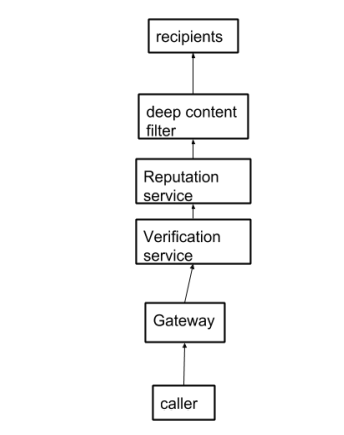
\includegraphics[width=15cm,height=20.5cm,keepaspectratio]{Capture.png} \\

The above diagram just summarizes the central idea behind the project’s backend. The real
architecture is much more complex and it is private to the Amazon.
When a customer desires to send an email he make a call to the main gateway, the service
that handles users requests. The gateway services redirects the call to other services in the
backend. The path that an email has to traverse to the recipients inbox is called sending
pipeline and works the following way:

\begin{enumerate}
\item The customer make an APi call to the gateway
\item The gateway redirects to email to a service that perfoms various verifications on the email, such as i the user is indeed eligible for sending
\item The reputation service decides if the email is going to be passed to the next node in the backend based on the reputation that this sender has. If a sender has low reputation, he's going to be allowed to send the email
\item The last node in the service checks if the email doesn't contain any malware or sensitive content
\item The email arrives in the customer's inbox
\end{enumerate}

This is the idea that an cloud email sending service is built on. Along side these services can
appear another services, for example services that collects metrics like when the sending of
an email failed due to bad reputation or failed the content filtering test.





\cite{Marc-2009}


\newpage

\begin{thebibliography}{9}

\bibliography{articles}
\bibitem{serf} 
https://www.serf.io/

\bibitem{orchestration}
https://www.mulesoft.com/resources/esb/service-orchestration-and-soa

\bibitem{orchestration2}
https://www.ciena.com/insights/what-is/what-is-service-orchestration.html

\bibitem{gitorchestraion}
https://github.com/hashicorp/serf/blob/master/README.md

\bibitem{article}
https://www.sciencedirect.com/science/article/pii/S016764230900029X

\bibitem{aws1}
https://aws.amazon.com/blogs/architecture/create-dynamic-contact-form

\bibitem{aws2}
https://aws.amazon.com/blogs/architecture/
\end{thebibliography}	


	
\end{document}